\documentclass{beamer}
\mode<presentation>
{
  \usetheme{myulm}
  \setbeamercovered{transparent}
  \setbeamertemplate{navigation symbols}{} % no navigation bar
  \setbeamersize{sidebar width left=1.17cm}
}

\usepackage[ngerman]{babel}
\usepackage[utf8]{inputenc}
\usepackage{amsmath,amssymb,amsfonts}
\usepackage{times}
\usepackage{graphicx}
\usepackage{fancyvrb}
\usepackage{array}
\usepackage{colortbl}

% Anfang der Titelfolie
% Anpassung von: Titel, Untertitel, Autor, Datum und Institut

\title{Kanonische Transformationen und die Hamilton-Jacobi-Gleichung}
\subtitle{Seminar I für Computationals Science and Engineering bei Prof. Lebiedz}
\author{Alexander Dürr und Anton Hügel}
\newcommand{\presdatum}{8. Februar 2018} % alternativ zu \today: Eingabe eines festen Datums
\institute
{\\Universität Ulm, Institut für Numerische Mathematik}
%Ende der Titelfolie

% Anfang der Kopfzeile der Folien
% Anpassung von: Zwischentitel, Leitthema oder Name
% Das Datum wird oben geändert: unter \presdatum{}!

\newcommand{\zwischentitel}{Zwischentitel}
\newcommand{\leitthema}{Lanczos Kap. 7 und 8}
% Ende der Kopfzeile

% Anfang der Folien
\begin{document}
\hspace*{-1.49cm}
\frame[plain]{\titlepage}

% Das Inhaltsverzeichnis
\hspace*{-0.7cm}
\begin{frame}
  \frametitle{Inhaltsverzeichnis}
  \tableofcontents
\end{frame}


\section{Bekanntes: Die kanonischen Gleichungen}

\section{Kanonische Transformationen}
    \begin{frame}
    \frametitle{Gesucht: Lösung der kanonischen Gleichungen}
    
    \begin{align*}
        \dot{q}_k &= \frac{\partial H}{\partial p_k} \\
        \dot{p}_k &= -\frac{\partial H}{\partial q_k}
    \end{align*}
    
    
\end{frame}

    \subsection{Lösung mechanischer Probleme mittels Koordinatentranformation}
    \begin{frame}
    \frametitle{Ausweg: Koordinatentransformation}
    
    Gesucht wird ein Koordinatensystem, indem die kanonischen Gleichungen direkt gelöst werden können.
    
    \begin{figure}
        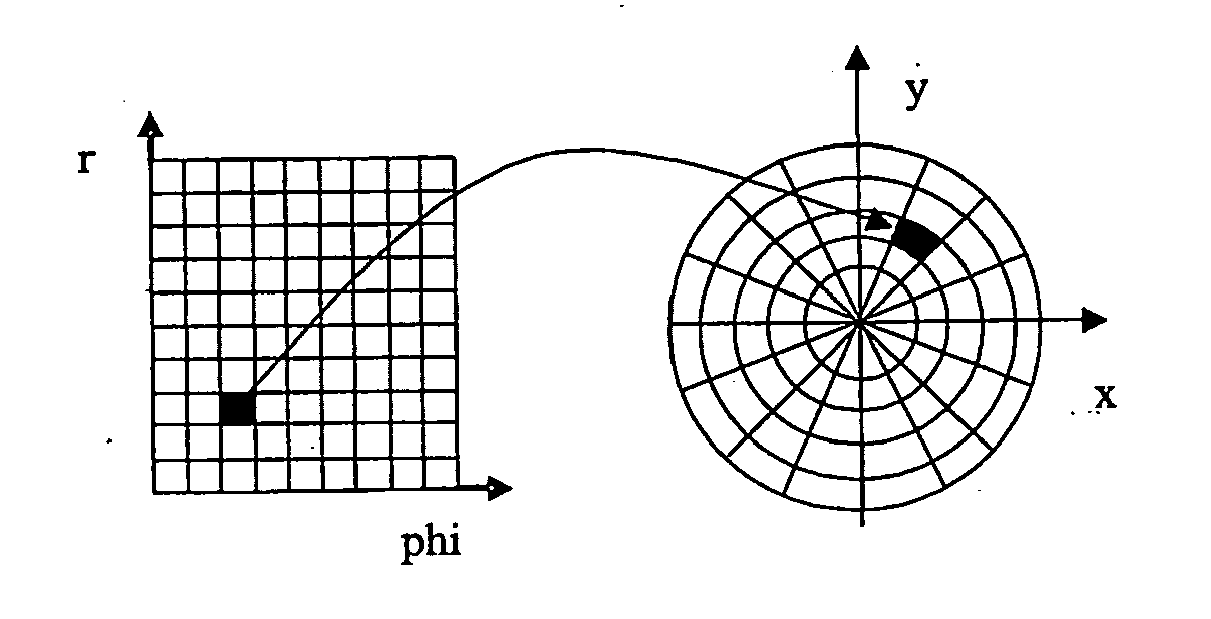
\includegraphics[scale=0.2]{images/koordtrans.png}
    \end{figure}
    
    
\end{frame}

\begin{frame}
    \frametitle{Ausweg: Koordinatentransformation}
    
    \textbf{Wichtig:} Lösungen müssen erhalten bleiben.\\
    D.h. wir brauchen Transformationen, gegenüber derer die kanonischen Gleichungen invariant sind. \\
    \vspace{5mm}    
    Solche Transformationen werden \emph{kanonische Transformationen} genannt.
    
    \begin{figure}
        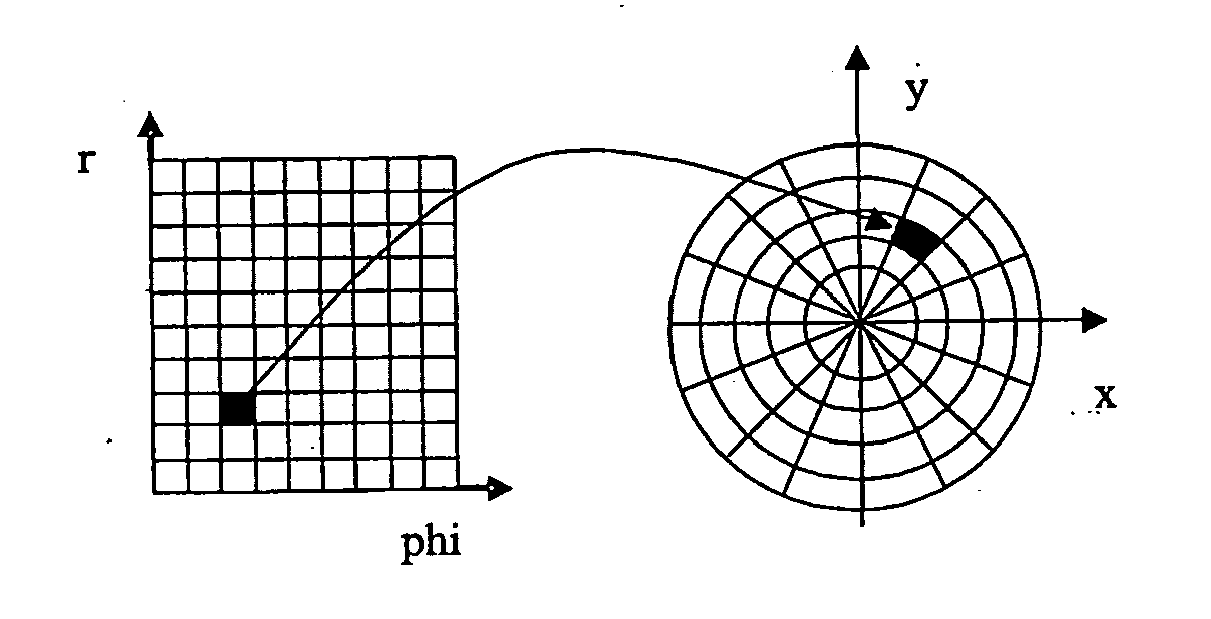
\includegraphics[scale=0.2]{images/koordtrans.png}
    \end{figure}
    
    
\end{frame}
    
    \subsection{Die Langrange'sche Punkttransformation}
    \begin{frame}
    \frametitle{Punkttransformation}
    
    Alte Koordinaten: $p_k, q_k$ \\
    Neue Koordinaten: $P_k, Q_k$
    
    Punkttransformationen haben die Form
    
    \begin{align*}
    q_1 &= f_1(Q_1,\ldots,Q_n) \\
        &\quad\vdots \\
    q_n &= f_n(Q_1,\ldots,Q_n)    
    \end{align*}
    
\end{frame}


    
    \subsection{Die allgemeine kanonische Transformation}
    \begin{frame}
    Die Invarianz von    
    \begin{displaymath}
            \sum_{i=1}^n p_i \delta q_i = \sum_{i=1}^n P_i \delta Q_i
    \end{displaymath}
    ist nicht notwendig. \\
    
    Allgemeinerer Ansatz:
    \begin{displaymath}
    \sum_{i=1}^n p_i \delta q_i = \sum_{i=1}^n P_i \delta Q_i + \delta S
    \end{displaymath}

\end{frame}

\begin{frame}

    Das kanonische Integral sieht nun folgendermaßen aus:
    
    \begin{align*}
    A &= \int_{t_1}^{t_2} \left( \sum_{i=1}^n p_i dq_i - H dt \right) \\
      &= \int_{t_1}^{t_2} \left( \sum_{i=1}^n P_i dQ_i - H dt \right)  +  \underbrace{\int_{t_1}^{t_2} dS}_{=\text{const.}}
    \end{align*}
    
    $\Longrightarrow$  Kannonische Gleichungen invariant unter dieser Transformation.
    
\end{frame}

\begin{frame}
    \frametitle{Allgemeine kanonische Transformation}
    
    
    \begin{displaymath}
        \sum_{i=1}^{n} (p_i \delta q_i - P_i \delta Q_i) = \delta S
    \end{displaymath}
    
    \begin{center} mit der generierenden Funktion $S = S(q_1,\ldots,q_n;Q_1,\ldots,Q_n)$ \end{center}
    
\end{frame}
    
    \subsection{Die bilineare Differentialform}
    \begin{frame}
    \frametitle{Die blineare Differenzialform}
    \begin{itemize}
        \item Jeder Transformation lässt bestimmte Größen unverändert
        \item Diese Invarianten bestimmen Eigenschaften der Transformation
        \item Für kanonische Transformation hatten wir zunächst $\sum p_i \delta q_i$
        \item Dann fanden wir die allgemeinere Bedingung     
                \begin{displaymath}
                \sum_{i=1}^{n} (p_i \delta q_i - P_i \delta Q_i) = \delta S
                \end{displaymath}
              Welcher Invarianten entspricht diese Bedingung?
    \end{itemize}
\end{frame}

\begin{frame}
   
        \begin{displaymath}
        \sum_{i=1}^{n} p_i \delta q_i - \sum_{i=1}^{n} P_i \delta Q_i = \delta S
        \end{displaymath}
        
        $\longrightarrow$ Erinnert an die Arbeit in einem monogenen (monogenic) System.\\
        \vspace{3mm}
        \emph{Masseteilchen wird auf beliebigem geschlossenen Pfad bewegt.\
              Ist die verrichtete Arbeit Null, wenn man wieder am Ausgangspunkt ankommt, so nennt man das System monogen.}
            
      \begin{center} 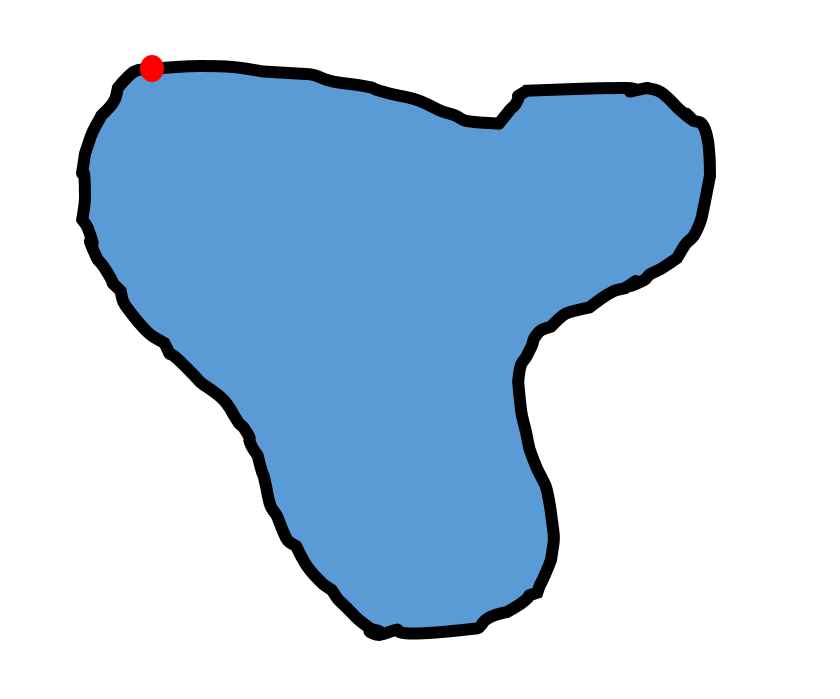
\includegraphics[scale=0.15]{images/monogenicSys}  \end{center}  
        
        

\end{frame}

\begin{frame}
    Integration von
    \begin{displaymath}
    \sum_{i=1}^{n} p_i d q_i - \sum_{i=1}^{n} P_i d Q_i = d S
    \end{displaymath}
    entlang einer geschlossenen Kurve ergibt.
   \begin{displaymath}
   \oint \sum_{i=1}^{n} p_i d q_i - \oint \sum_{i=1}^{n} P_i d Q_i = 0
   \end{displaymath}
    \begin{center} 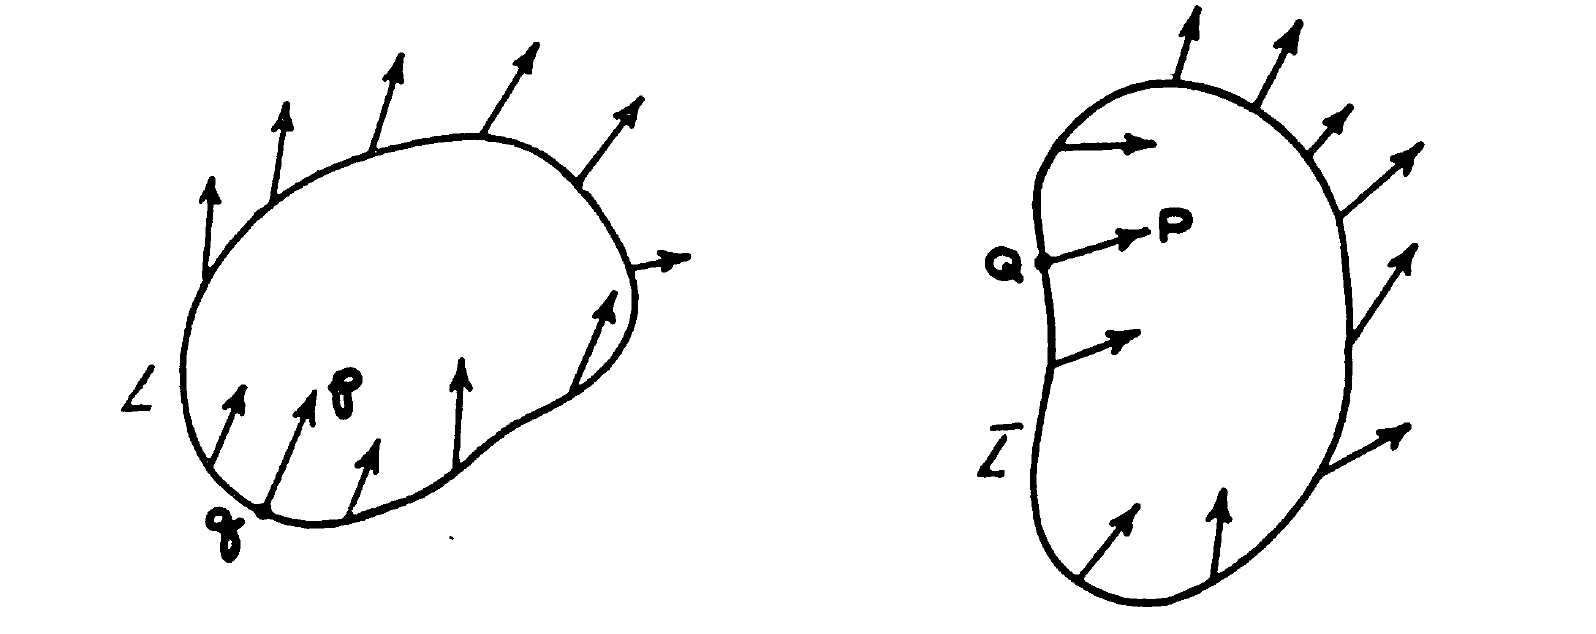
\includegraphics[scale=0.225]{images/circulation}  \end{center}  

\end{frame}

\begin{frame}
     \emph{Für jede geschlossene Kurve im Phasenraum ist}
    \begin{displaymath}
    \Gamma = \oint \sum_{i=1}^{n} p_i d q_i = \oint \sum_{i=1}^{n} P_i d Q_i
    \end{displaymath}
     \emph{eine Invariante gegenüber der kanonischen Transformationen.}
 
\end{frame}
    
    \subsection{Lagrange Klammer}
    \begin{frame}
    \frametitle{Lagrange- und Poisson-Klammer}

    Seien $q_i$ und $p_i$ zwei Koordinatensysteme, $u$ und $v$ Parameter. \\

    \begin{align*}
    \textbf{Lagrange-Klammer: } \qquad    [u,v] = \sum_{i=1}^{n} \left(   \frac{\partial q_i}{\partial u} \frac{\partial p_i}{\partial v} - \frac{\partial q_i}{\partial v} \frac{\partial p_i}{\partial u}  \right)  \\
    \textbf{Poisson-Klammer: } \qquad    (u,v) = \sum_{i=1}^{n} \left(   \frac{\partial u}{\partial q_i} \frac{\partial v}{\partial p_i} - \frac{\partial v}{\partial q_i} \frac{\partial u}{\partial p_i}  \right)  
    \end{align*}

\end{frame}

\begin{frame}
    Es gilt:
    \vspace{5mm}
    \begin{itemize}
        \item Die kanonischen Transformationen sind diejenigen Transformationen von $q_i,p_i$ zu $Q_i,P_i$, für welche die \emph{Lagrange-Klammer} invariant ist.
        \vspace{5mm}
        \item Die kanonischen Transformationen sind diejenigen Transformationen von $q_i,p_i$ zu $Q_i,P_i$, für welche die \emph{Poisson-Klammer} invariant ist.
    \end{itemize}
    
\end{frame}

    
    \subsection{Gruppeneigenschaft}
    \begin{frame}
    \frametitle{Kanonische Transformationen sind Gruppe}
    
    Zwei kanonische Transformationen:
    \begin{align*}
        \sum_{i=1}^{n} (p_i \delta q_i - P_i \delta Q_i) &= \delta S \\
        \sum_{i=1}^{n} (P_i \delta Q_i - \bar{p}_i \delta \bar{q}_i) &= \delta \bar{S}
    \end{align*}
    
    Summe ist wieder kanonische Transformation:
        \begin{align*}
        \sum_{i=1}^{n} (p_i \delta q_i - \bar{p}_i \delta \bar{q}_i) &= \delta (S + \bar{S}) 
        \end{align*}
        
    Für jedes $S=S(q_1,\ldots,q_n; Q_1,\ldots,Q_n;t),\quad t>0$ gibt es eine Transformation.
    
\end{frame}


\begin{frame}
    \begin{align*}
        t,&\qquad t+\Delta t \\
        Q_k &= q_k + \Delta q_k \\
        P_k &= p_k + \Delta p_k
    \end{align*}
    
    \begin{align*}
        \Longrightarrow \qquad \Delta q_i &= \frac{\partial B}{\partial p_i} \Delta t,\\
                         \Delta p_i &= -\frac{\partial B}{\partial q_i} \Delta t
    \end{align*}
    
    mit
    
    \begin{displaymath}
        B(q_1,\ldots,q_n; p_1,\ldots,p_n;t) = \frac{\partial S}{\partial t}
    \end{displaymath}
\end{frame}

\begin{frame}
\hspace*{-2.2cm}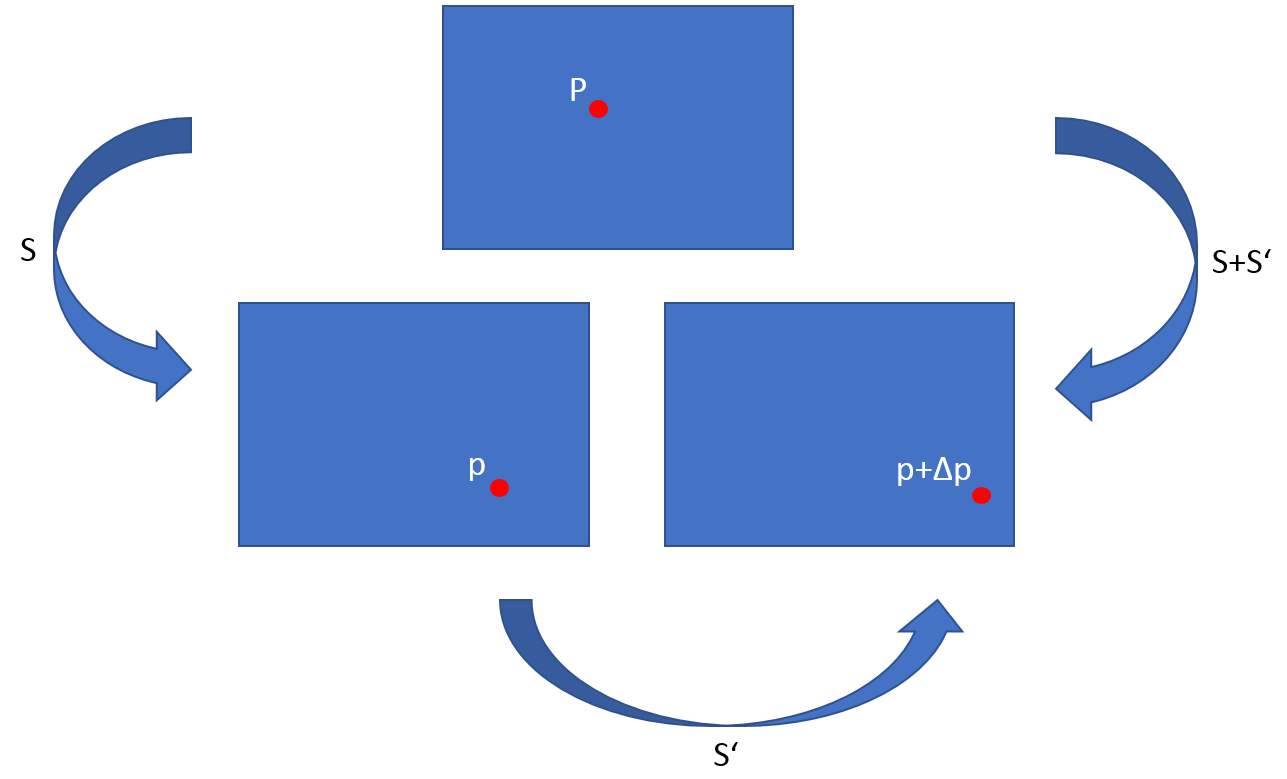
\includegraphics[scale=0.375]{images/ImagTrans}
\end{frame}

\begin{frame}
    \begin{align*}
    \Delta q_i &= \frac{\partial B}{\partial p_i} \Delta t,\\
    \Delta p_i &= -\frac{\partial B}{\partial q_i} \Delta t \\[5mm]
      \Delta t &\longrightarrow 0 \\[5mm]
    \frac{dq_i}{dt}  &= \frac{\partial B}{\partial p_i},\\
    \frac{dp_i}{dt} &= -\frac{\partial B}{\partial q_i} 
    \end{align*}
    
    $\rightarrow$ Das sind die kanonischen Bewegungsgleichungen.

\end{frame}
    
    \subsection{Infinitesimale kanonische Transformationen}
    
    \subsection{Das Phasenfluid als kanonische Transformationen}
    
    
\section{Die Hamilton-Jacobi-Gleichung}

    \subsection{Jacobis Transformationstheorie}
    
    \subsection{Lösung durch Separation}
    
    \subsection{Partielle Differenzialgleichungen bei Hamilton und Jacobi}

    \subsection{Geometrische Lösung und Wellenanalogie}

\section{Zusammenfassung}


\end{document}